\chapter{龍與獸的權勢，羔羊得勝（12:1–14:20）}

啟示錄第12至13章大量引用或呼應創世記與但以理\idx{07}{但以理}書的異象。若忽略這些舊約背景，我們很容易按照自己的想像解讀，甚至誤解經文的意思。因此，本章將帶領讀者從舊約出發，認識這些異象的背景與象徵，進而理解啟示錄所描繪的屬靈爭戰，以及敵對神的勢力如何與神的救贖\idx{11}{救贖}計畫相抗衡。

那麼，屬神的子民為什麼能勝過魔鬼呢？啟示錄12:11給出了關鍵的一句話：「弟兄勝過他，是因羔羊\idx{10}{羔羊}的血，和自己所見證的道。」基督徒所面對的爭戰，不只是看得見的人事物，也涉及更深的屬靈爭戰。因此，教會的得勝\idx{11}{得勝}不是靠自己的力量擊敗龍，而是因著羔羊的血，並在苦難中仍然持守所見證的道。

接著，第14章描繪天使在天上傳揚永遠的福音\idx{05}{永遠的福音}，呼召地上的人敬畏神，將榮耀\idx{14}{榮耀}歸給祂。為什麽到了這個時候，神還要差派天使給人傳福音？

在這短暫的世上，什麼能存留到永恆？
正是接受神浩大的恩典\idx{10}{恩典}，並且蒙召忠心跟隨基督。基督徒在地上為主作工、為主作見證、培育門徒，都是福分。正如啟示錄14:13所說：「他們息了自己的勞苦，作工的果效也隨著他們。」這提醒我們，為主所作的工不會徒然；即使信徒在世上經歷苦難，仍可以存著盼望，忠心持守到底。

為了幫助讀者掌握這些異象的背景與意義，同時不偏離「羔羊的得勝」這一主題，我整理了以下表格，放在此章的開始，讓讀者先對相關異象、舊約出處及其象徵意義有整體的認識。

{
\small
\renewcommand{\arraystretch}{1}
\setlength{\tabcolsep}{4pt}

\begin{longtable}{
  p{0.21\textwidth}
  p{0.25\textwidth}
  p{0.39\textwidth}
}
\caption{啟示錄12--13章異象的舊約背景}
\label{tab:rev12-13-ot-background-zh} \\
\hline
啟示錄異象 &
舊約背景 &
象徵意義\\
\hline
\endfirsthead

啟示錄異象 &
舊約背景 &
象徵意義 \\
\hline
\endhead

婦人 &
創 37:9-11；賽 54:1-8；66:7-9 &
以色列\idx{05}{以色列}與神的約民 \\

龍 &
創 3:1-15 &
古蛇、撒但\idx{15}{撒但}，以及敵對神的勢力 \\

七頭十角 &
但 7:7-8、24 &
象徵敵對神的帝國權勢 \\

男孩子 &
詩 2:7-9 &
彌賽亞君王耶穌基督 \\

鐵杖 &
詩 2:9 &
彌賽亞統治萬國 \\

一千二百六十天\idx{01}{一千二百六十天}、四十二個月、三年半\idx{03}{三年半} &
但 7:25；12:7 &
一段有限的受苦時期；敵對神的勢力受神限制 \\

天上爭戰 &
但 10:13、20-21；12:1 &
天上屬靈爭戰的背景 \\

海獸\idx{10}{海獸} &
但 7:2-8 &
敵對神及神的子民的帝國權力 \\

十角 &
但 7:7、24 &
君王的政治權勢 \\

地獸\idx{06}{地獸} &
但7章；啟13:11 &
模仿羔羊的外貌，卻傳達龍的權勢，迷惑世人 \\

額上與手上的記號 &
出 13:9、16；申 6:8；11:18 &
神子民將神的話記在手上與額上；
獸的印記\idx{19}{獸的印記}呈現對獸的歸屬與效忠 \\

666 & &
象徵敵對神的權勢及其不完全
\\
\hline
\end{longtable}
}

\begin{ReaderQuestion}
表\ref{tab:rev12-13-ot-background-zh}中幾乎每一個象徵都根源於舊約。將啟示錄與聖經其他部分一同閱讀，如何能保護我們免於揣測或誤解？
\end{ReaderQuestion}

\section{婦人：以色列}

\begin{ScriptureBox2}{圈出婦人和龍各自的樣子。龍等著要做什麼？}

\item[12:1] 天上現出大異象來．有一個婦人、身披日頭、腳踏月亮、頭戴十二星的冠冕．

\item[12:2] 他懷了孕、在生產的艱難中疼痛呼叫。

\item[12:3] 天上又現出異象來．有一條大紅龍、七頭十角、七頭上戴著七個冠冕。

\item[12:4] 他的尾巴拖拉著天上星辰的三分之一、摔在地上．龍就站在那將要生產的婦人面前、等他生產之後、要吞喫他的孩子。

\end{ScriptureBox2}

\begin{figure}[htbp]
    \centering
    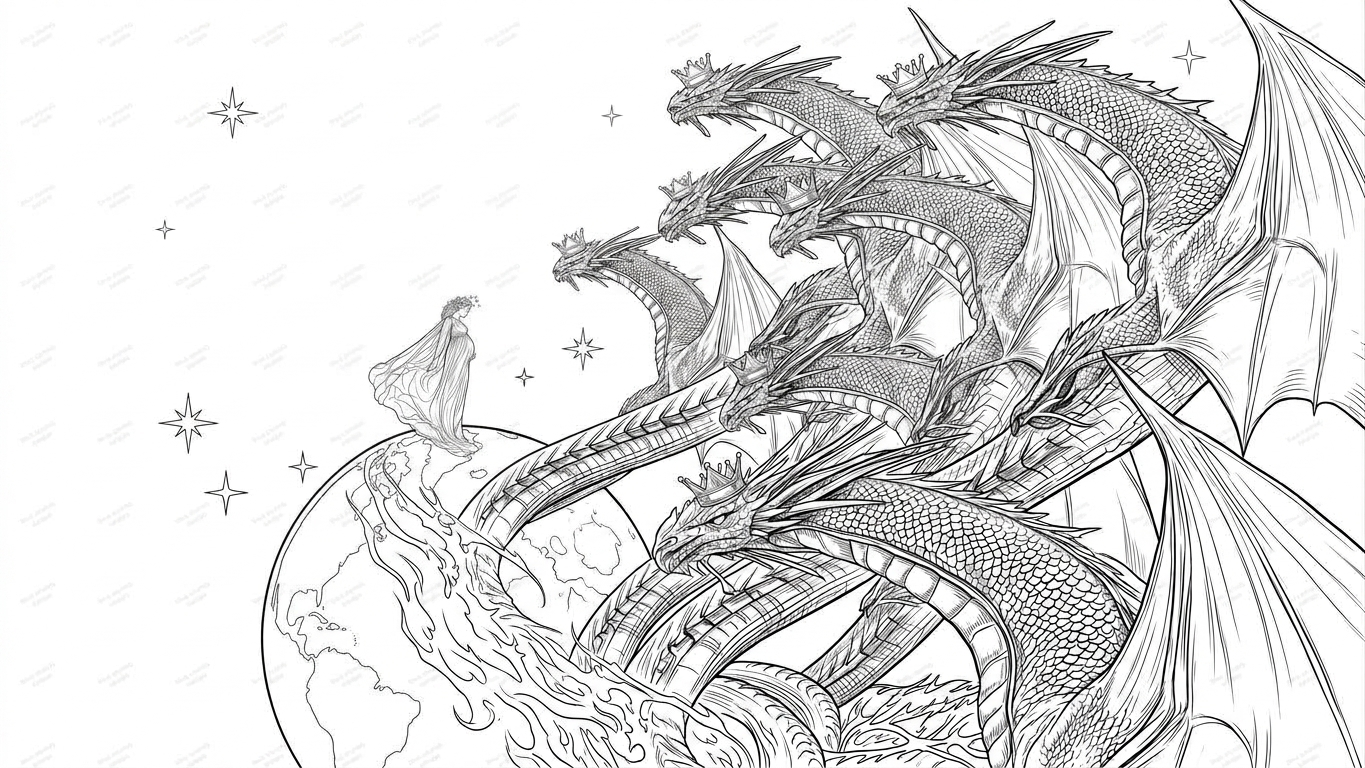
\includegraphics[
    width=1\textwidth, 
    trim=0 0 0 0, 
    clip]{images/woman_and_dragon2.jpg}
\end{figure}

此婦人身披日頭、腳踏月亮、頭戴十二星的冠冕，很容易讓熟悉聖經的讀者想到創世記37:9–11約瑟的夢。夢中出現太陽、月亮和十一顆星，分別代表雅各、拉結與約瑟的十一個哥哥；連同約瑟自己，十二顆星也使人聯想到以色列\idx{05}{以色列}十二支派。
此外，以賽亞\idx{05}{以賽亞}書多次將神的子民或錫安描寫成婦人，描繪神與祂子民的關係（賽 26:17–18；49:14–23；54:1–8；66:7–9）。
尤其是以賽亞66:7-9說「婦人尚未劬勞就生產」，
所以這裡的婦人應當廣義的代表以色列及神的約民。\footnote{G. K. Beale, The Book of Revelation: A Commentary on the Greek Text (Grand Rapids, MI: Eerdmans, 1999), 625.}

當然，由於婦人生下的男孩子是彌賽亞耶穌基督，也有人將婦人理解為耶穌的母親馬利亞。然而，日頭、月亮、頭戴十二星的異象，似乎是廣義的以色列比較妥當。


\section{男孩子：耶穌基督}

\begin{ScriptureBox2}{這男孩子將來要做什麼？他被提到哪裡去了？}

\item[12:5] 婦人生了一個男孩子、是將來要用鐵杖轄管萬國的．〔轄管原文作牧〕他的孩子被提到　神寶座那裡去了。

\end{ScriptureBox2}

這裡直接引用詩篇2:7-9：「你是我的兒子，我今日生你……你必用鐵杖打破他們……」所以男孩子即是彌賽亞君王，是基督。

這裡從男孩子的出生，就接著是龍對男孩子的攻擊，然後就直接說結局「男孩子被提到神寶座\idx{20}{寶座}」，而省略了降生、受死、復活、升天。是把救贖\idx{11}{救贖}歷史事件高度濃縮了。
約翰的焦點不是要講耶穌地上的生平，而是要說龍沒有能力消滅神所立的彌賽亞君王。
\footnote{這正是「預表性／救贖歷史性」的讀法。
預表性：看舊約的人物、事件或制度如何預先指向基督。
救贖歷史性（redemptive-historical）：把經文放在神救贖計畫的整條時間線上來讀，看這段經文在創造、墮落、救贖、成全中位於哪個階段。重點是「進程」。}

\begin{ScriptureBox2}{劃出12:11中弟兄勝過那控告者的三個原因。婦人如何得保護、躲避那龍？龍接著去與誰爭戰？}

\item[12:6] 婦人就逃到曠野、在那裡有　神給他預備的地方、使他被養活一千二百六十天。

\item[12:7] 在天上就有了爭戰．米迦勒同他的使者與龍爭戰．龍也同他的使者去爭戰．

\item[12:8] 並沒有得勝、天上再沒有他們的地方。

\item[12:9] 大龍就是那古蛇、名叫魔鬼、又叫撒但、是迷惑普天下的．他被摔在地上、他的使者也一同被摔下去。

\item[12:10] 我聽見在天上有大聲音說、我　神的救恩、能力、國度、並他基督的權柄、現在都來到了．因為那在我們　神面前晝夜控告我們弟兄的、已經被摔下去了。

\item[12:11] 弟兄勝過他、是因羔羊的血、和自己所見證的道．他們雖至於死、也不愛惜性命。

\item[12:12] 所以諸天和住在其中的、你們都快樂罷．只是地與海有禍了、因為魔鬼知道自己的時候不多、就氣忿忿的下到你們那裡去了。

\item[12:13] 龍見自己被摔在地上、就逼迫那生男孩子的婦人。

\item[12:14] 於是有大鷹的兩個翅膀賜給婦人、叫他能飛到曠野、到自己的地方、躲避那蛇．他在那裡被養活一載二載半載。

\item[12:15] 蛇就在婦人身後、從口中吐出水來像河一樣、要將婦人沖去。

\item[12:16] 地卻幫助婦人、開口吞了從龍口吐出來的水。〔原文作河〕

\item[12:17] 龍向婦人發怒、去與他其餘的兒女爭戰、這兒女就是那守　神誡命、為耶穌作見證的。那時龍就站在海邊的沙上。

\end{ScriptureBox2}


\begin{figure}[htbp]
    \centering
    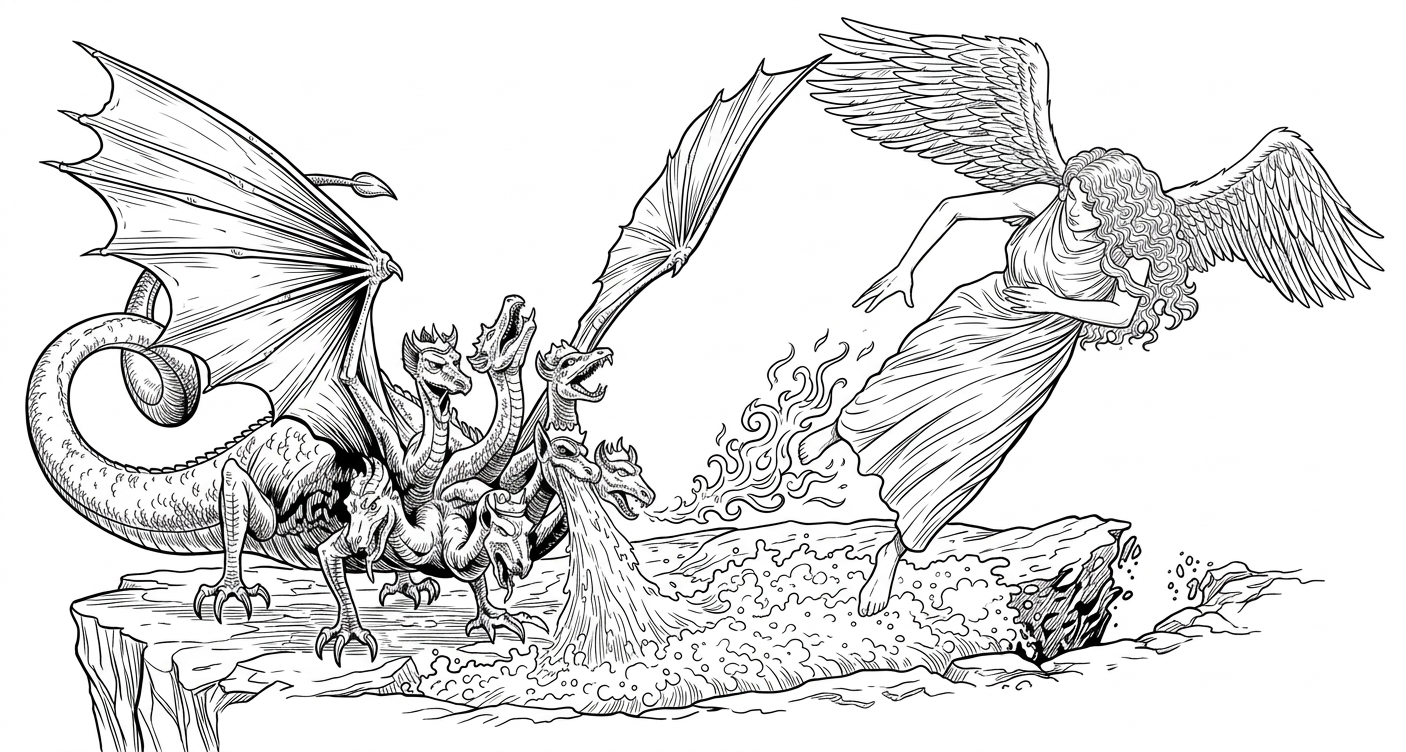
\includegraphics[
    width=1\textwidth, 
    trim=0 0 0 0, 
    clip]{images/woman_fly_away.jpg}
\end{figure}


「一千二百六十天\idx{01}{一千二百六十天}」，是三年半\idx{03}{三年半}（1260/360 = 3.5）。但以理\idx{07}{但以理}書有多處提到三年半。不過如果我們試圖去用某一個世代的三年半來解釋，就常常變得牽強而且失去焦點。最好的解釋就是字面的解釋，是神限制了獸的時間。在此三年半，婦人受神的保護，之後，龍被摔下去，並加緊逼迫\idx{13}{逼迫}婦人和她其餘的兒女。

\begin{ReaderQuestion}
龍的怒氣越來越大，但牠的時候受神限制，婦人也在曠野被養活。當你面對一段似乎越來越艱難、而非逐漸緩和的試煉時期，知道神為它設定了界限，並且一路扶持你，會如何改變你忍耐的方式？
\end{ReaderQuestion}

\section{海獸：地上敵對神的帝國權勢}


\begin{ScriptureBox2}{圈出這獸所像的動物。誰把能力給了這獸？牠可以任意而行多久？}

\item[13:1] 我又看見一個獸從海中上來、有十角七頭、在十角上戴著十個冠冕、七頭上有褻瀆的名號。

\item[13:2] 我所看見的獸、形狀像豹、腳像熊的腳、口像獅子的口．那龍將自己的能力、座位、和大權柄、都給了他。

\item[13:3] 我看見獸的七頭中、有一個似乎受了死傷．那死傷卻醫好了。全地的人、都希奇跟從那獸．

\item[13:4] 又拜那龍、因為他將自己的權柄給了獸．也拜獸說、誰能比這獸、誰能與他交戰呢。

\item[13:5] 又賜給他說誇大褻瀆話的口．又有權柄賜給他、可以任意而行四十二個月。

\item[13:6] 獸就開口向　神說褻瀆的話、褻瀆　神的名、並他的帳幕、以及那些住在天上的。

\item[13:7] 又任憑他與聖徒爭戰、並且得勝．也把權柄賜給他、制伏各族各民各方各國。

\item[13:8] 凡住在地上、名字從創世以來、沒有記在被殺之羔羊生命冊上的人、都要拜他。

\item[13:9] 凡有耳的、就應當聽。

\item[13:10] 擄掠人的必被擄掠．用刀殺人的、必被刀殺。聖徒的忍耐和信心、就是在此。

\end{ScriptureBox2}

「獸」象徵地上的帝國勢力。這是我們從但以理\idx{07}{但以理}書得知的。
但以理書第七章敘述有四個獸從海中上來，但以理書並且解釋那四個獸就是在世上興起的四個王。
接著但以理書第八章以公綿羊與公山羊的異象，預言瑪代波斯與希臘的興起，以及希臘君王的崛起與後續帝國的分裂。\footnote{通常被認為是亞歷山大大帝（但以理書 8:21）。亞歷山大大帝於主前四世紀征服波斯，是約在但以理兩百年之後。}
所以「獸」是指地上的帝國勢力。

這裡的啟示錄，龍被摔下去之後，就站在海邊的沙上。它開始做什麼呢？
它結合海上來的獸與地上來的獸。這裡的海獸\idx{10}{海獸}代表什麼呢？它直接對應但以理書七章。

這裡的「海」代表多國多民。根據啟示錄17:15的解釋，「眾水」就是「多民、多人、多國、多方」。
因此，海獸從「海」中上來，代表從列國中興起、並敵對神和祂子民的地上權勢。
此海獸直接對應但以理書7章的描述。

我製表\ref{tab:rev13-daniel7-zh}來對應此處的異象在兩書中的章節。
{
\renewcommand{\arraystretch}{1}
\small
\begin{longtable}{p{3cm} p{3.5cm} p{2.7cm}}
\caption{啟示錄13章的獸與但以理書7章的四獸}
\label{tab:rev13-daniel7-zh} \\
\hline
啟示錄13 &
但以理書7 &
代表 \\
\hline
1 獸從海中上來 &
2-3 四獸從海上來 &
列國帝國 \\
2 獸有像獅子的口 &
4 第一獸像獅子 &
獅子的意象 \\
2 獸有像熊的腳 &
5 第二獸像熊 &
熊的意象 \\
2 獸的形狀像豹 &
6 第三獸像豹 &
豹的意象 \\
1 可怕權勢 &
7 第四獸極其可怕 &
勝過過去的帝國\\
1 獸有十角 &
7 第四獸有十角 &
帝國性權力 \\
6 獸說褻瀆的話 &
8 小角說誇大的話 &
僭越神的權柄 \\
7 獸與聖徒爭戰 &
21 小角與聖民爭戰 &
逼迫\idx{13}{逼迫}神子民 \\
7 獸「得勝\idx{11}{得勝}」 &
21 小角「勝了他們」 &
暫時性勝利 \\
羔羊\idx{10}{羔羊}最終審判\idx{15}{審判}獸 &
22 「亙古常在者」 &
最終審判 \\
5 四十二個月 &
25 一載、二載、半載 &
逼迫時期有限制 \\
7 任憑獸與聖徒爭戰 &
25 聖民交在獸手中 &
神容許但限制其權勢 \\
獸面對神的審判 &
26-27 獸的權柄最終被除滅 &
獸終必敗亡 \\
\hline
\end{longtable}
}

\begin{ReaderQuestion}
在表\ref{tab:rev13-daniel7-zh}中，啟示錄13章的獸結合了但以理書7章四獸的特徵：獅子、熊、豹和十角。牠甚至「勝過聖徒」，但表格最後卻以牠的權柄被除滅作結。今天世上有哪些權勢在你看來顯得強大或可怕？這個表如何幫助你從神最終審判的角度來看待它們？
\end{ReaderQuestion}

更讓人驚訝的是，龍把權柄給海獸，這海獸受傷又醫好了，結果全地的人都希奇跟從那獸。這裡形成一個很明顯的基督受死又復活的仿冒者。
真正的基督是受死、復活、得榮耀\idx{14}{榮耀}，可是這海獸是似乎死、卻恢復、然後得到普世敬拜。


\begin{figure}[htbp]
    \centering
    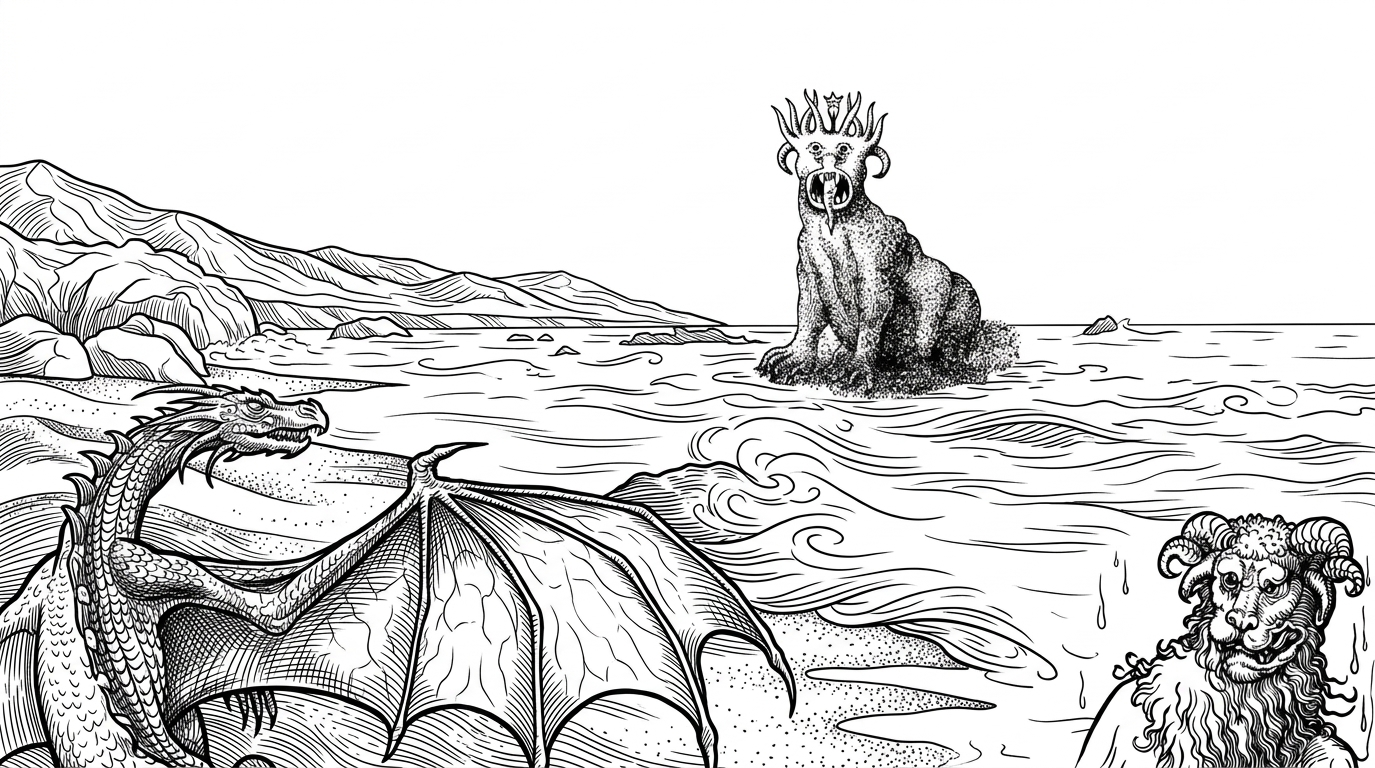
\includegraphics[
    width=1\textwidth, 
    trim=0 0 0 0, 
    clip]{images/dragon_and_breast.jpg}
\end{figure}

\section{從地上來的獸：假先知}

\begin{ScriptureBox2}{第二個獸是什麼樣子？牠說話像什麼？劃出牠叫住在地上的人所做的一切事。}

\item[13:11] 我又看見另有一個獸從地中上來．有兩角如同羊羔、說話好像龍。

\item[13:12] 他在頭一個獸面前、施行頭一個獸所有的權柄．並且叫地和住在地上的人、拜那死傷醫好的頭一個獸。

\item[13:13] 又行大奇事、甚至在人面前、叫火從天降在地上。

\item[13:14] 他因賜給他權柄在獸面前能行奇事、就迷惑住在地上的人、說、要給那受刀傷還活著的獸作個像。

\item[13:15] 又有權柄賜給他叫獸像有生氣、並且能說話、又叫所有不拜獸像的人都被殺害。

\end{ScriptureBox2}

現在我們來看地上的獸。它有像羔羊\idx{10}{羔羊}的外表，但說話像龍。所以這是一個欺騙性的宗教。啟示錄16:13、19:20、20:10後來稱它為假先知\idx{11}{假先知}。

\begin{ReaderQuestion}
地獸外貌像羔羊，說話卻像龍。這提醒我們如何分辨表面敬虔、實際上卻迷惑人的教導？
\end{ReaderQuestion}

因此地獸\idx{06}{地獸}不是單純另一個政治帝國，而是依附在第一獸的統治下行神蹟、欺騙人、推動敬拜獸、使人接受獸的印記\idx{19}{獸的印記}。

所以龍、海獸\idx{10}{海獸}、地獸，形成一個假冒的三位一體\idx{11}{假冒的三位一體}。龍模仿神，獸模仿羔羊，假先知模仿聖靈的工作。

\begin{ReaderQuestion}
龍、海獸與地獸如何彼此配合，形成對神的模仿與敵對？這對我們認識屬靈爭戰有什麼幫助？
\end{ReaderQuestion}

\section{人的數目：666}

\begin{ScriptureBox2}{誰被迫受印記？印記在哪裡？沒有印記的人不能做什麼？}

\item[13:16] 他又叫眾人、無論大小貧富、自主的為奴的、都在右手上、或是在額上、受一個印記。

\item[13:17] 除了那受印記、有了獸名、或有獸名數目的、都不得作買賣。

\item[13:18] 在這裡有智慧。凡有聰明的、可以算計獸的數目．因為這是人的數目、他的數目是六百六十六。

\end{ScriptureBox2}

受了獸的印記\idx{19}{獸的印記}的人，才能夠做買賣。而在此段期間出生的，不接受獸的印記的神的僕人，是不能做買賣的。
因此不接受獸的印記的神的僕人，所受到的逼迫\idx{13}{逼迫}是很大的。他們受到嚴重的經濟排斥，甚至可能必須依靠以物易物的方式維持生活。

但是他們持守真理，只有被殺的羔羊\idx{10}{羔羊}配得敬拜，祂的子民靠著羔羊的血與忠心見證，在獸的逼迫中得勝\idx{11}{得勝}。

為什麼是「666」而不是「777」？這裡比較不適合用666去解釋某種密碼。
我們知道聖經中「7」常與完整、圓滿有關。「666」卻是三重的「不完全」，這裡形成一種強烈的對比：神的完全是「7」，而獸的極度自我高舉是「666」。

有人把獸的印記與當代科技、條碼、晶片、身分證或無現金支付等聯繫起來；這些可以作為現代人的聯想，卻不能直接當作啟示錄對未來科技的預言。經文真正強調的，是對獸的敬拜、效忠，以及由此產生的社會與經濟逼迫。

\begin{ReaderQuestion}
獸的印記與神子民對神的忠心有什麼對比？當信仰與經濟利益或社會壓力發生衝突時，我們應當如何持守信仰？
\end{ReaderQuestion}


\section{羔羊與祂的百姓同在}

龍、海獸\idx{10}{海獸}、地獸\idx{06}{地獸}，形成的假冒的三位一體\idx{11}{假冒的三位一體}的異象令人震撼。
然而，第14章把我們的目光重新帶回羔羊\idx{10}{羔羊}。

約翰看見羔羊站在錫安山，與祂同在的有十四萬四千人\idx{02}{十四萬四千人}。他們額上寫著羔羊和祂父的名，表明他們真正所屬的不是獸，而是神。他們跟隨羔羊，無論祂往哪裡去；他們在患難中仍然持守神的誡命和耶穌的真道。

第13章的假冒的三位一體，與第14章真正的羔羊，成為一個重要的對比。獸要求人敬拜牠，可是我們看見羔羊的百姓敬拜祂。世界可能用權勢、恐懼和利益逼迫\idx{13}{逼迫}人妥協，但神認得屬祂的人。

接著，三位天使宣告審判\idx{15}{審判}已經來到。第一位天使宣告永遠的福音\idx{05}{永遠的福音}，呼召萬民敬畏神、將榮耀\idx{14}{榮耀}歸給祂；第二位宣告巴比倫\idx{04}{巴比倫}傾倒；第三位警告拜獸的人將面對神的審判。最後，兩幅收割\idx{06}{收割}的圖畫把我們帶到歷史的終局：莊稼成熟了，葡萄也熟透了，神的審判必然來到。

然而，在這些嚴肅的審判信息中，神特別賜下一句安慰：

「從今以後，在主裡面而死的人有福了。」

他們雖然在地上經歷勞苦，甚至為基督而死，但他們的勞苦並沒有徒然。他們「息了自己的勞苦」，「作工的果效也隨著他們」。


\begin{ScriptureBox2}{十四萬四千人的額上寫著什麼？劃出14:4–5中描述他們的每一句話。}
\item[14:1] 我又觀看、見羔羊站在錫安山、同他又有十四萬四千人、都有他的名、和他父的名、寫在額上。

\item[14:2] 我聽見從天上有聲音、像眾水的聲音、和大雷的聲音．並且我所聽見的好像彈琴的所彈的琴聲。

\item[14:3] 他們在寶座前、並在四活物和眾長老前唱歌、彷彿是新歌．除了從地上買來的那十四萬四千人以外、沒有人能學這歌。

\item[14:4] 這些人未曾沾染婦女、他們原是童身。羔羊無論往那裡去、他們都跟隨他。他們是從人間買來的、作初熟的果子歸與　神和羔羊。

\item[14:5] 在他們口中察不出謊言來．他們是沒有瑕疵的。

\end{ScriptureBox2}



%\begin{figure}[htbp]
%    \centering
%    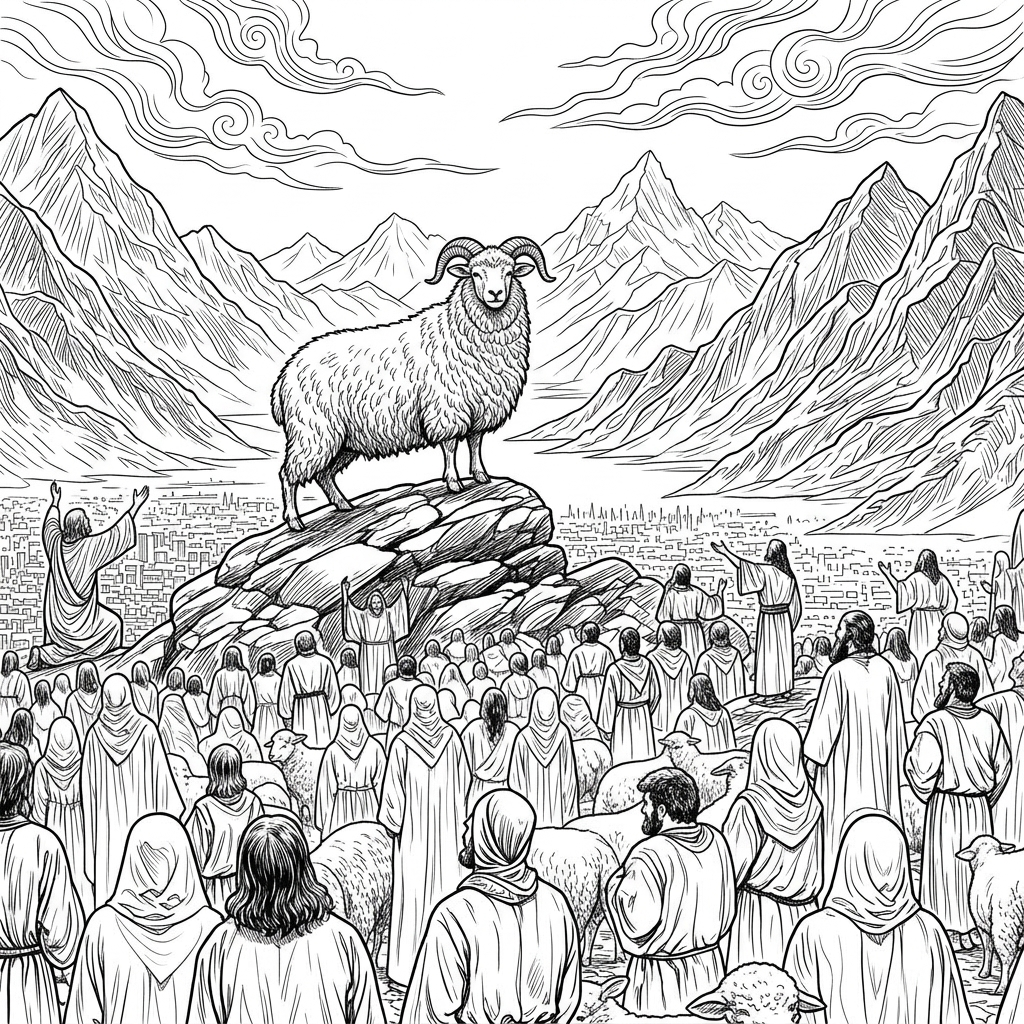
\includegraphics[
%    width=1\textwidth, 
%    trim=0 0 0 0, 
%    clip]{images/lamb_14400.jpg}
%\end{figure}


他們是「從人間買來的、作初熟的果子歸與　神和羔羊」，表示他們也是被耶穌救贖\idx{11}{救贖}的人。「在他們口中察不出謊言來．他們是沒有瑕疵的」是說在耶穌的眼中，他們是
沒有瑕疵的。
他們是「未曾沾染婦女、他們原是童身」的，可能就是獨身，沒有沾染婦女者。
因為舊約以婚姻與淫亂描寫對神忠誠或不忠，這裡表示，他們是忠誠於羔羊的人。無論羔羊往那裡去、他們都跟隨他。

\begin{ReaderQuestion}
「羔羊無論往那裡去，他們都跟隨他」（14:4）對你而言意味著什麼？
\end{ReaderQuestion}

他們的歌，有天地間的獨特。是只有親身走過救贖之路、在考驗中堅定跟隨羔羊的人，才能從靈魂深處唱出的生命讚美。沒有人能學他們的新歌。

\section{天使傳永遠的福音}

\begin{ScriptureBox2}{劃出三位天使各自宣告的內容。14:13中誰是有福的？為什麼？}


\item[14:6] 我又看見另有一位天使飛在空中、有永遠的福音要傳給住在地上的人、就是各國各族各方各民．

\item[14:7] 他大聲說、應當敬畏　神、將榮耀歸給他．因他施行審判的時候已經到了．應當敬拜那創造天地海和眾水泉源的。

\item[14:8] 又有第二位天使、接著說、叫萬民喝邪淫大怒之酒的巴比倫大城傾倒了、傾倒了。

\item[14:9] 又有第三位天使、接著他們、大聲說、若有人拜獸和獸像、在額上、或在手上、受了印記、

\item[14:10] 這人也必喝　神大怒的酒、此酒斟在　神忿怒的杯中純一不雜．他要在聖天使和羔羊面前、在火與硫磺之中受痛苦．

\item[14:11] 他受痛苦的煙往上冒、直到永永遠遠．那些拜獸和獸像受他名之印記的、晝夜不得安寧。

\item[14:12] 聖徒的忍耐就在此．他們是守　神誡命、和耶穌真道的。

\item[14:13] 我聽見從天上有聲音說、你要寫下、從今以後、在主裡面而死的人有福了．聖靈說、是的、他們息了自己的勞苦、作工的果效也隨著他們。

\end{ScriptureBox2}

\begin{figure}[h]
    \centering
    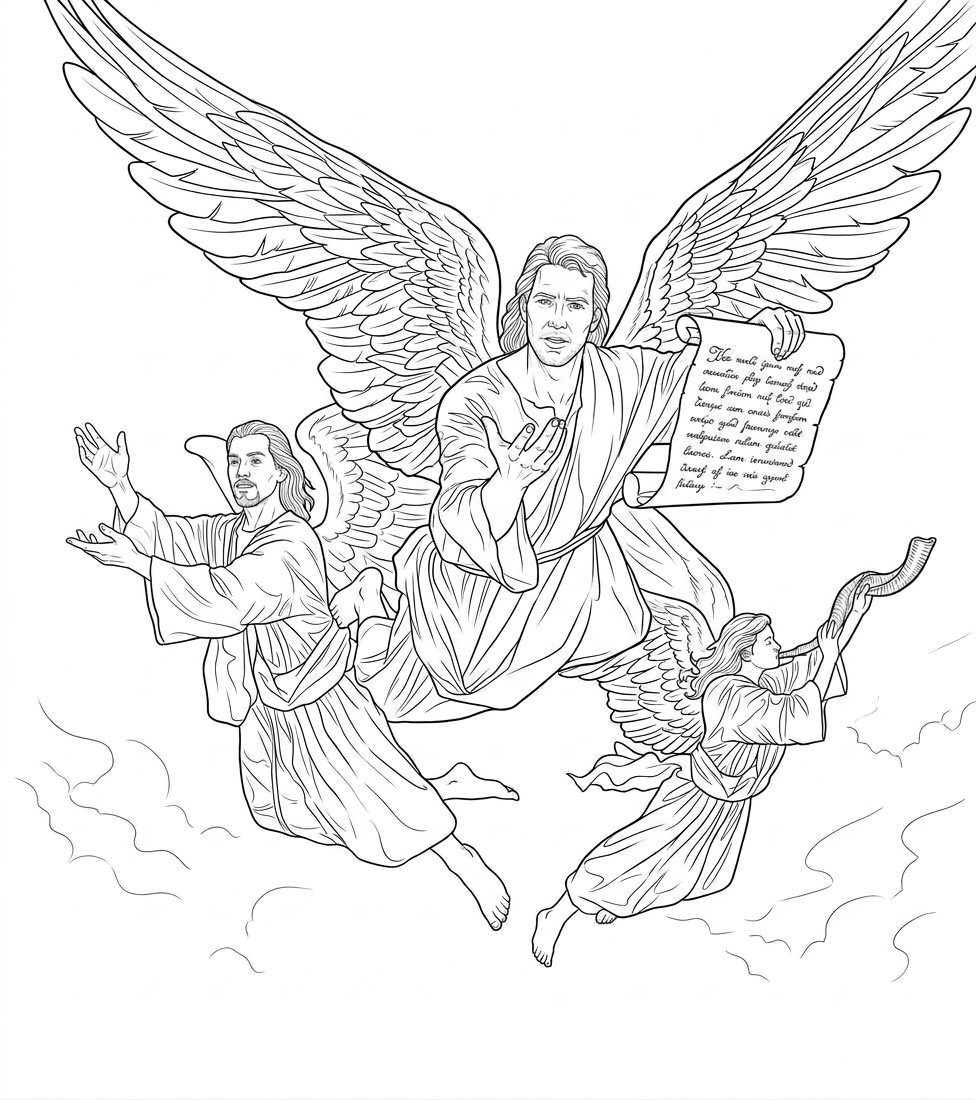
\includegraphics[
    width=0.8\textwidth, 
    trim=0 0 0 0, 
    clip]{images/eternal_gospel.jpg}
\end{figure}

到了這個時候，天上仍然有福音傳給地上的人。這福音是什麼呢？就是人應當要「敬畏神，將榮耀\idx{14}{榮耀}歸給他」，要敬拜祂，因為祂是「創造天地海和眾水泉源的。」
人受造，就是生命的恩典\idx{10}{恩典}，人敬拜神並歸榮耀與神，是受造之人應當對造物主回應。

\begin{ReaderQuestion}
第一位天使所宣告的「永遠的福音」包括哪些內容？（14:6–7）為什麼「敬畏神、將榮耀歸給祂、敬拜創造主」與福音的信息有關？
\end{ReaderQuestion}

接著其他兩位天使宣判公義的審判\idx{15}{審判}。悖逆的受造之人不只拒絕受造之恩典，
拒絕耶穌的救贖\idx{11}{救贖}的寶血，
而且拜獸，在手上接受印記，逼迫\idx{13}{逼迫}聖徒。所以拜獸之人受痛苦，直到永永遠遠，這樣的審判豈不公義嗎？

而忍耐持守的人，在主裡面而死的人，有福了。他們真的息了自己的勞苦，他們一生為主做工的果效也隨著他們，這是多大的安慰！

\section{兩幅收割的異象}


\begin{ScriptureBox2}{比較這兩次收割。誰揮出第一把鐮刀？第二次收割收取的是什麼？又被丟在哪裡？}

\item[14:14] 我又觀看、見有一片白雲、雲上坐著一位好像人子、頭上戴著金冠冕、手裡拿著快鐮刀。

\item[14:15] 又有一位天使從殿中出來、向那坐在雲上的大聲喊著說、伸出你的鐮刀來收割．因為收割的時候已經到了、地上的莊稼已經熟透了。

\item[14:16] 那坐在雲上的、就把鐮刀扔在地上．地上的莊稼就被收割了。

\item[14:17] 又有一位天使從天上的殿中出來、他也拿著快鐮刀。

\item[14:18] 又有一位天使從祭壇中出來、是有權柄管火的、向拿著快鐮刀的大聲喊著說、伸出快鐮刀來收取地上葡萄樹的果子．因為葡萄熟透了。

\item[14:19] 那天使就把鐮刀扔在地上、收取了地上的葡萄、丟在　神忿怒的大酒醡中。

\item[14:20] 那酒醡踹在城外、就有血從酒醡裡流出來、高到馬的嚼環、遠有六百里。

\end{ScriptureBox2}

前面幾章我們已經講過，這裡的「人子\idx{02}{人子}」就是耶穌基督。莊稼已經熟了，所以祂手裡拿著快鐮刀要收割\idx{06}{收割}了。
耶穌在約翰福音4:35說：「你們豈不說、到收割的時候、還有四個月麼．我告訴你們、舉目向田觀看、莊稼已經熟了、〔原文作發白〕可以收割了。」
滿滿金黃色的麥子低垂，工人們拿著快鐮刀收割，這是多麼快樂的場景！

收割的時候，也是審判\idx{15}{審判}的時候。工人們會將麥子和稗子分別開來，麥子收在倉裡，稗子燒掉。
這就是主耶穌在馬太福音13:24-30，用農家最能夠了解的比喻，
農夫不需要在幼苗的時候就分別麥子和稗子。要容許這兩樣一齊長。在收割的時候，就可以分別出來。\footnote{馬太福音13:24-30：「耶穌又設個比喻對他們說、天國好像人撒好種在田裡．
及至人睡覺的時候、有仇敵來、將稗子撒在麥子裡、就走了。
到長苗吐穗的時候、稗子也顯出來。
田主的僕人來告訴他說、主阿、你不是撒好種在田裡麼、從那裡來的稗子呢。
主人說、這是仇敵作的。僕人說、你要我們去薅出來麼。
主人說、不必、恐怕薅稗子、連麥子也拔出來。
容這兩樣一齊長、等著收割．當收割的時候、我要對收割的人說、先將稗子薅出來、捆成捆、留著燒．惟有麥子、要收在倉裡。」}

收割和審判，在約珥書3:13講的明明白白：「開鐮罷．因為莊稼熟了．踐踏罷。因為酒醡滿了、酒池盈溢．他們的罪惡甚大。」
啟示錄這裡有天使把鐮刀扔在地上，是要收取地上的葡萄，然後丟在神忿怒的大酒醡中。審判的時候到了。
審判罪大惡極的惡人，就像醡葡萄酒一樣，酒池盈溢流出，竟然高至馬的嚼環，遠達六百里。

\begin{ReaderQuestion}
啟示錄14章呈現兩次收割：人子收割的莊稼，以及被丟在神忿怒大酒醡中的葡萄。既然最後的收割還沒有來到，神今天的忍耐應當如何影響你回應祂的方式，以及你向別人談論祂的方式？
\end{ReaderQuestion}

\begin{figure}[htbp]
    \centering
    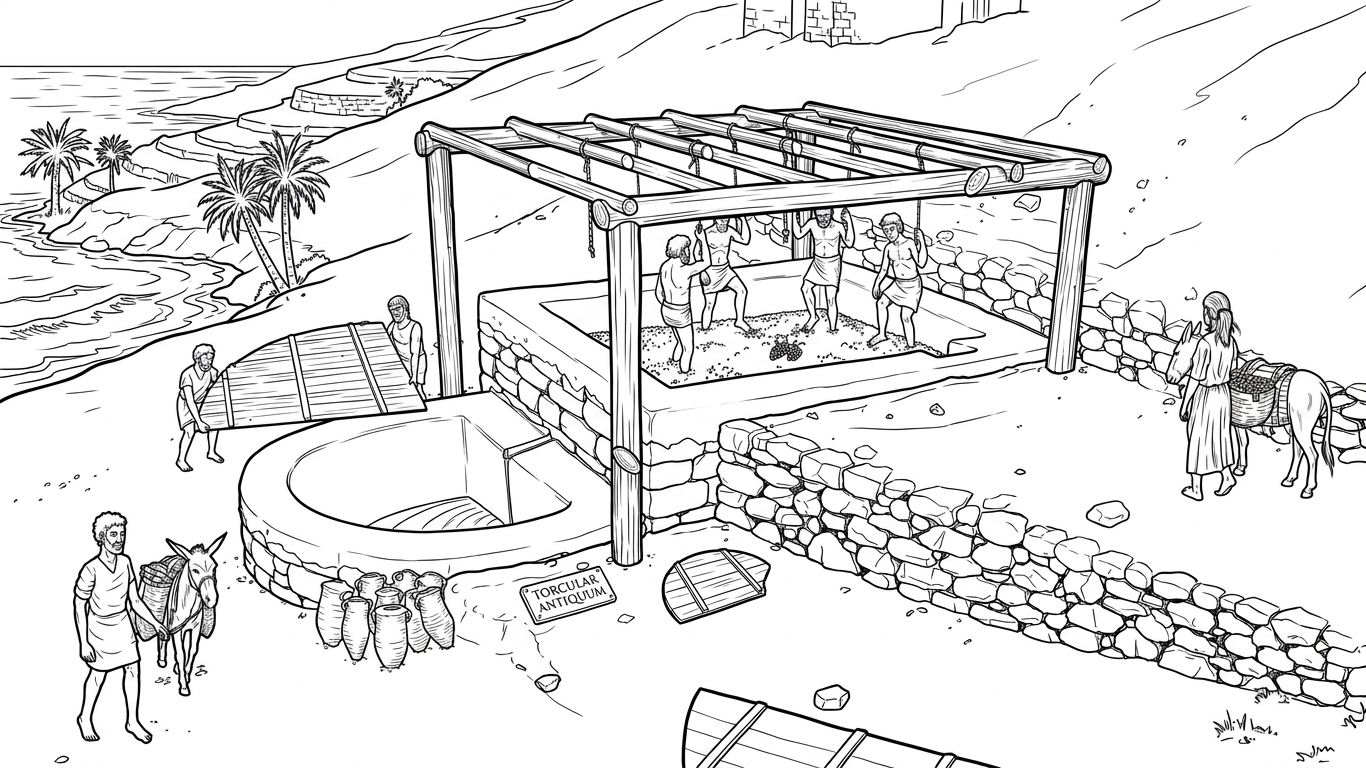
\includegraphics[
    width=1\textwidth, 
    trim=0 0 0 0, 
    clip]{images/wine_pressing.jpg}
\end{figure}
